\documentclass{article}
\usepackage{graphicx}
\usepackage{subcaption}
\usepackage[font=small,labelfont=bf]{caption}
\begin{document}
	
	\title{Taxi time dependency on runway and parking area}
	\maketitle
\section*{Introduction}
We explored the dependency of taxi time on the runway and on the parking area, with a particular focus on Air France and FedEx flights. 

We expect the taxi time to be larger when the distance between the parking slot and the runway is larger. This is especially evident with FedEx flight, since they all leave from the same parking area (called I), situated at the periphery of the airport platform.
\section{Airport Structure}
\begin{figure}[h]
	\centering
	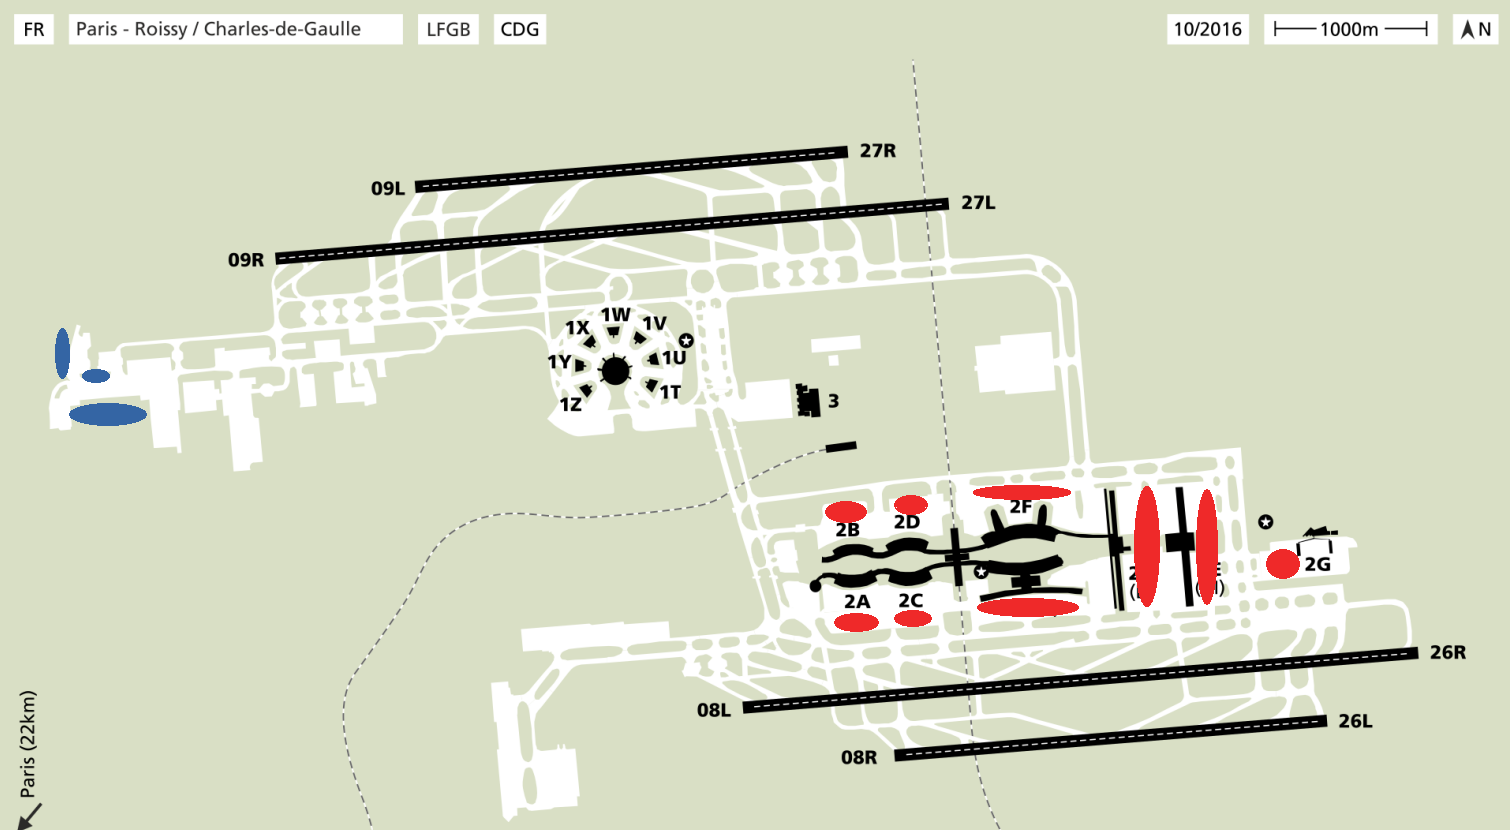
\includegraphics[width=\textwidth]{map_airport_filled}
	\caption{Map of Charles de Gaulle airport. The red ovals correspond to the gates where Air France aircrafts usually park. The blue ovals correspond where FedEx aircrafts park.}
	\label{map}
\end{figure}

Figure ~\ref{map} shows a map of the entire airport, where the parking areas for FedEx and AirFrance aircrafts are evidenced.

We can see from the map that Air France aircrafts have a quicker access to the runways, expecially the southern ones, since their parking position is central. FedEx aircraft, on the other side, have a quite quick access to the northern runways only when they are taking off facing east or landing facing west. While the large distance from the southern runways might be a reason for delay.

\subsection{The runways}
To better understand the variations in taxi time, it's essential to explain the standard use of the four runways, that take different names based on whether the aircrafts face east or west. 
\begin{center}
	
\begin{tabular}{c|c|c|c}
	\centering
	\textbf{Runway} & \textbf{Airport zone} & \textbf{Facing} & \textbf{Movement}\\
	\hline
	09L & North & East & Arrival \\
	27R & North & West & Arrival \\
	09R & North & East & Departure\\
	27L & North & West & Departure\\
	08R & South & East & Arrival\\
	26L & South & West & Arrival\\
	08L & South & East & Departure\\
	26R & South & West & Departure\\	
\end{tabular}
\end{center}

\section{Air France flights}
To see if there were significant differences in the taxi times of Air France flights based on the runway, we computed the mean and the standard deviation of taxi times for all the runways.


\begin{table}[h!!!!!!!!!!!!!!!!!]	
	\centering
	\begin{tabular}{c|c|c|c}
		\centering
		\textbf{Runway} & \textbf{Mean taxi time (s)} & \textbf{$\sigma$ (s)} & Frequency\\
		\hline
		08R & 305 & 184 & 13\%\\
		\hline
		26R & 344 & 221 & 22\%\\
		\hline
		26L & 386 & 154 & 20\%\\
		\hline
		08L & 426 & 270 & 16\%\\
		\hline
		09L & 480 & 190 & 6\%\\
		\hline
		27L & 511 & 284 & 10\%\\
		\hline
		27R & 660 & 211 & 6\%\\
		\hline
		09R & 766 & 334 & 7\%\\	
	\end{tabular}
\caption{Taxi time avaraged over a total of 511791 Air France flights, relative standard deviation and relative frequency of usage of that runway ordered by increasing mean.}
\label{tableRunway}
\end{table}
It is evident from the table \ref{tableRunway} that the taxi time is shorter for southern runways for Air France flights: this is explained by the shorter distance between southern runways and Air France parking areas.
Moreover, we performed an ANOVA test to verify if the difference between the taxi times for different runways were statistically significant, resulting in a strong evidence that they are (p-value lower than $10^{-15}$).


\begin{figure}[h!!!!!!!!]
	\centering
	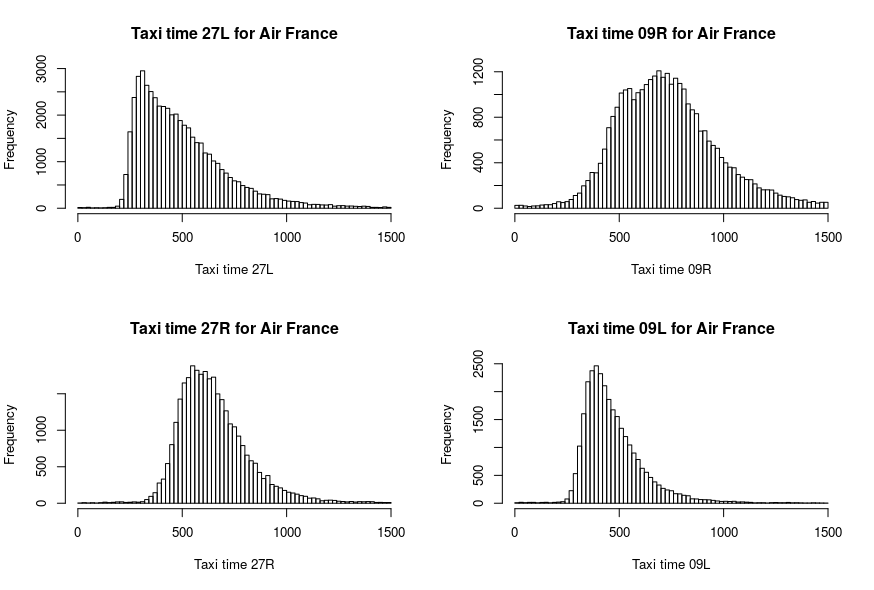
\includegraphics[width=10cm]{AFR_pistes_nord}
	\caption{Distribution of taxi times for Air France flights for the northern runways.}
	\label{distN}
\end{figure}
\begin{center}
\begin{figure}[h!!!!!!!!]
	\centering
	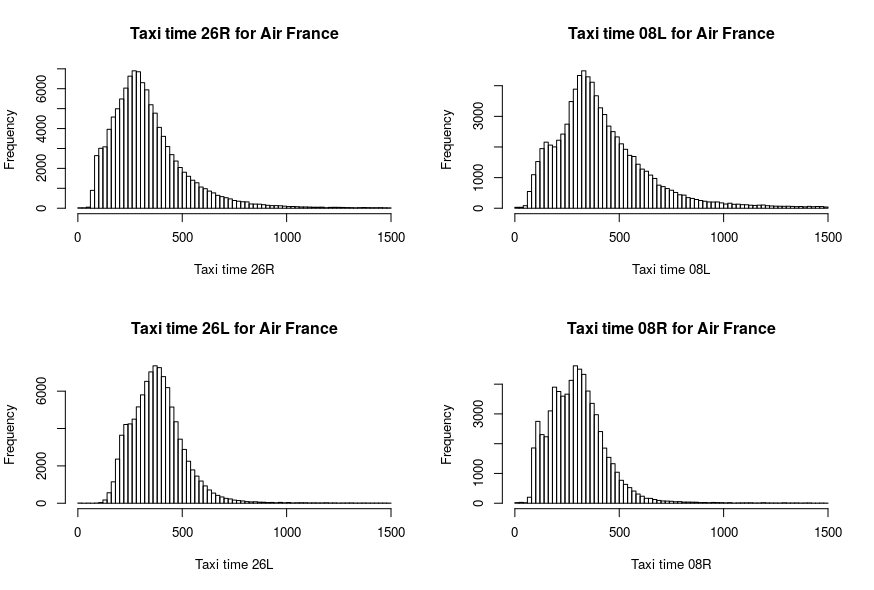
\includegraphics[width=10cm]{AFR_pistes_sud}
	\caption{Distribution of taxi times for Air France flights for the northern runways.}
	\label{distS}
\end{figure}
\end{center}


\newpage

We plotted the distribution of taxi times for Air France flights grouped by runway in Figures \ref{distN} and \ref{distS}.

\section{FedEx flights}
We analysed FedEx flights to be able to explain the peak in the taxi time at 3 a.m. In fact, from approximately 1:30 a.m. to 3:30 a.m., most of the flights are from FedEx or its partners, like ASL Airlines Ireland.

We present below the table and the histograms analogous to those showed for Air France.



\begin{table}[h!!!!!!!!!!!!!!!!!]	
	\centering
	\begin{tabular}{c|c|c|c}
		\centering
		\textbf{Runway} & \textbf{Mean taxi time (s)} & \textbf{$\sigma$ (s)} &  \textbf{Frequency}\\
		\hline
		27R & 325 & 155 & 26 \% \\
		\hline
		09R & 340 & 217 & 17\%\\
		\hline
		09L & 536 & 138 & 19\%\\
		\hline
		26L & 666 & 203 & 2\%\\
		\hline
		27L & 680 & 247& 20\%\\
		\hline
		08L & 828 & 262 & 7\%\\
		\hline
		08R & 832 & 238 & 1\%\\
		\hline
		26R & 1099 & 314 & 8\%\\	
	\end{tabular}
	\caption{Taxi time avaraged over a total of 23832 FedEx flights, relative standard deviation and relative frequency of usage of that runway ordered by increasing mean.}
	\label{tableRunwayFDX}
\end{table}

As expected, we see that the mean taxi time is low only for the runways dedicated to the take off facing east and to the landing facing west.
As in the case of Air France flights, the ANOVA test suggested that the taxi times for different runways are significantly different.

In Figures \ref{distNFDX} and \ref{distSFDX} the distributions for taxi times for different runways are shown.

\begin{figure}[h!!!!!!!!]
	\centering
	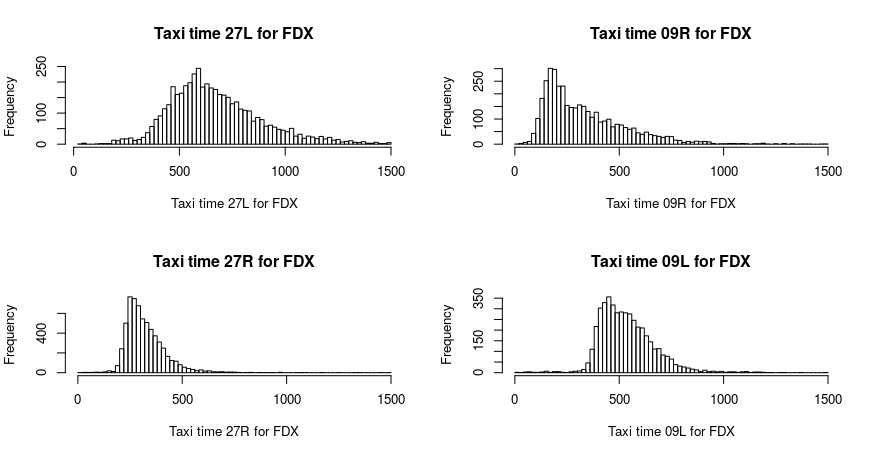
\includegraphics[width=\textwidth]{FDX_pistes_nord}
	\caption{Distribution of taxi times for FedEx flights for the northern runways.}
	\label{distNFDX}
\end{figure}

\begin{center}
	\begin{figure}[h!!!!!!!!]
		\centering
		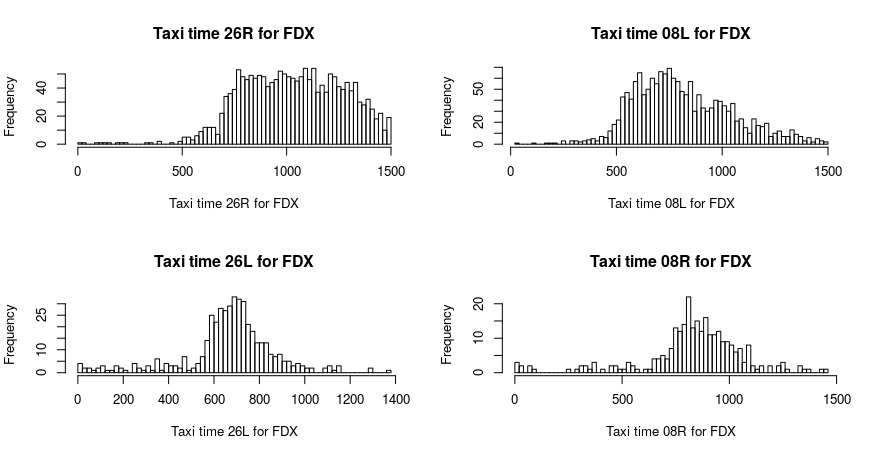
\includegraphics[width=\textwidth]{FDX_pistes_sud}
		\caption{Distribution of taxi times for FedEx flights for the southern runways.}
		\label{distSFDX}
	\end{figure}
\end{center}

\section{Comments and future work}
As expected, the mean taxi time increases as the distance between the parking slot and the runway increases.

What can be further analyzed are the non-Gaussian shapes of some of the distributions presented. In fact, for what it concerns FedEx flights, this can partly be imputed to the low number of observations. But for what it concerns Air France flights, we can see that some of the curves, such as the ones for runways 09R, 26R, 08L and 08R, look like the sum of two or more Gaussians. It would be interesting to isolate the factors that cause this kind of shapes.




\end{document}